\section*{Exercise 2}
\subsection*{Data-related questions}

a. \textbf{Briefly describe the CIFAR-10 dataset used in this implementation, incl. the types of images and categories.}\\
The CIFAR-10 dataset contains 60,000 color images (32x32 pixels) across 10 classes, with 6,000 images per class. It is split into 50,000 training images and 10,000 test images.
The training data is organised into five batches of 10,000 images each, while the test set is one batch of 10,000 images (1,000 from each class). Each class is distinct with no overlap between categories.\\
The 10 classes are:
\begin{enumerate}
	\item airplane
	\item automobile
	\item bird
	\item  cat
	\item  deer
	\item  dog
	\item rog
	\item horse
	\item ship
	\item ruck
\end{enumerate}
b. \textbf{What are the transformations used for data augmentation?} \\
Before training the model, two main data augmentation techniques are applied. Images are randomly cropped to size 32x32 with a padding of 4. This simulates zooming and shifting, making the model less sensitive to the exact position of objects. Images are also randomly flipped horizontally, which helps the model generalise better to mirrored versions of objects.
In addition, all images are  normalised using the dataset's mean and standard deviation for the training and testing data.

These augmentations increase the diversity of the training data and reduce the risk of overfitting, since the model cannot rely on memorizing specific pixel arrangements. Instead, it learns more general patterns.
\subsection*{Model-related questions}

a. What is an optimizer? What is the initial learning rate? You can change the value of the initial learning rate and check how it affects the model performance (fast or slow convergence). You can select two different learning rates, one is larger and the other is
smaller than the default setting and plot the training curves. \\

An optimizer is an algorithm used to adjust the weights and biases during training to minimize the loss function which tells us how far the model's predictions are from the true values.

The initial learning rate is a hyperparameter that determines the step size the optimizer takes when updating the model's parameters regarding the gradient and loss function. A large learning rate can lead to faster initial convergence, but risks overshooting the minimum which can lead to not reaching an optimal solution. A small learning rate leads to more stable convergence, but delays the training process and risks getting stuck in a local minimum. 

Below you can find a short analysis where a larger (0.3) and a smaller (0.03) learning rate were considered, the default one being 0.1 .

\begin{figure}[H]
    \centering
    \begin{subfigure}[t]{0.48\textwidth}
        \centering
        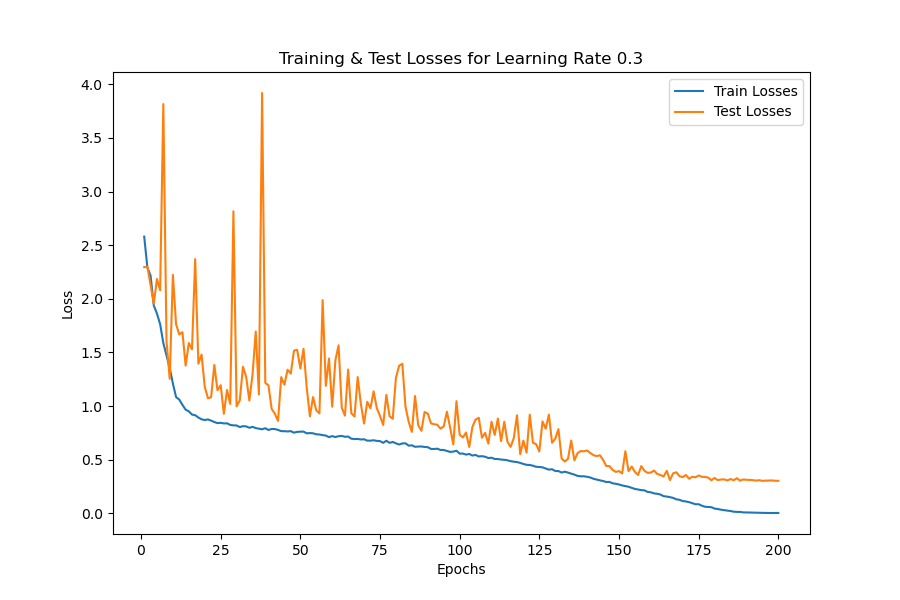
\includegraphics[width=\textwidth]{assignment_1/report/images/losses_03.png}
        \caption{Average training vs. test loss per epoch for learning rate 0.3.}
    \end{subfigure}
    \hfill
    \begin{subfigure}[t]{0.48\textwidth}
        \centering
        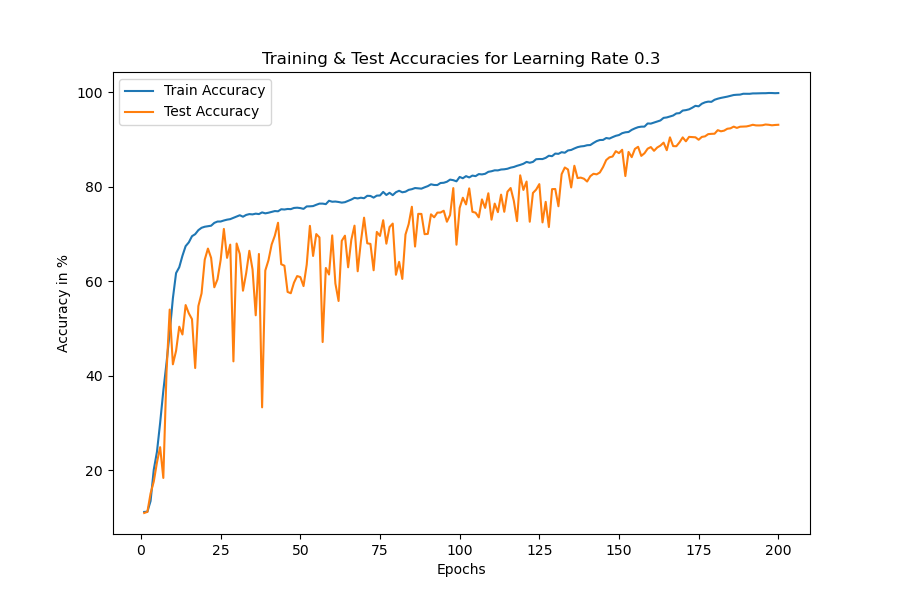
\includegraphics[width=\textwidth]{assignment_1/report/images/accuracies_03.png}
        \caption{Average training vs. test accuracy per epoch for learning rate 0.3.}
    \end{subfigure}
    \caption{Training and testing performance metrics with learning rate 0.3.}
\end{figure}

\begin{figure}[H]
    \centering
    \begin{subfigure}[t]{0.48\textwidth}
        \centering
        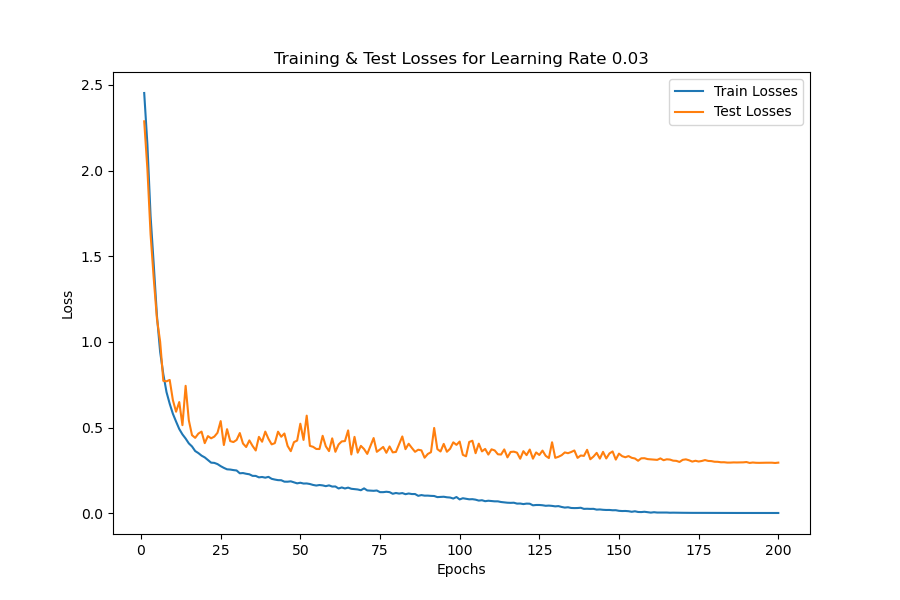
\includegraphics[width=\textwidth]{assignment_1/report/images/losses_003.png}
        \caption{Average training vs. test loss per epoch for learning rate 0.03.}
    \end{subfigure}
    \hfill
    \begin{subfigure}[t]{0.48\textwidth}
        \centering
        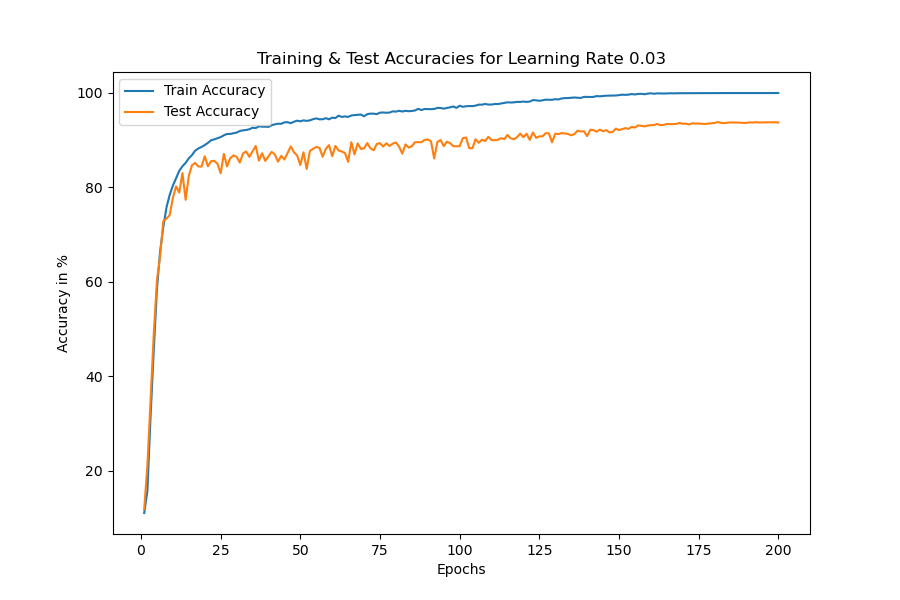
\includegraphics[width=\textwidth]{assignment_1/report/images/accuracies_003.png}
        \caption{Average training vs. test accuracy per epoch for learning rate 0.03.}
    \end{subfigure}
    \caption{Training and testing performance metrics with learning rate 0.03.}
\end{figure}

\textbf{Larger Learning Rate 0.3}

Both the test loss and test accuracy are very volatile, fluctuating especially in the first 100 epochs. The loss convergence is slow and noisy which indicates that the optimizer is overshooting the minimum repeatedly.

\textbf{Smaller Learning Rate 0.03}

Both the loss and accuracy convergence are smooth showing a stable training process. The test loss stabilizes on a lower consistent value than the larger learning rate.

\begin{table}[h]
    \centering
    \caption{Effect of Learning Rate on Model Convergence}
    \begin{tabular}{|c|c|c|c|}
        \hline
        \textbf{Learning Rate} & \textbf{Effect on Convergence} & \textbf{Test Loss Volatility} & \textbf{Final Test Accuracy} \\
        \hline
        $0.3$ (Larger) & Noisy and Unstable & High & $\approx 93\%$ \\
        \hline
        $0.03$ (Smaller) &  Smooth and Stable & Low & $\approx 94\%$ \\
        \hline
    \end{tabular}
\end{table}

b. Confirm the size of the feature maps after each convolution block. Display the feature maps. You can show 3 images of the 2D feature maps from 3 different convolutional blocks: the first, the last and one in between that is up to your choice. In total, you will have 9 images.

\begin{figure}[H] 
    \centering
    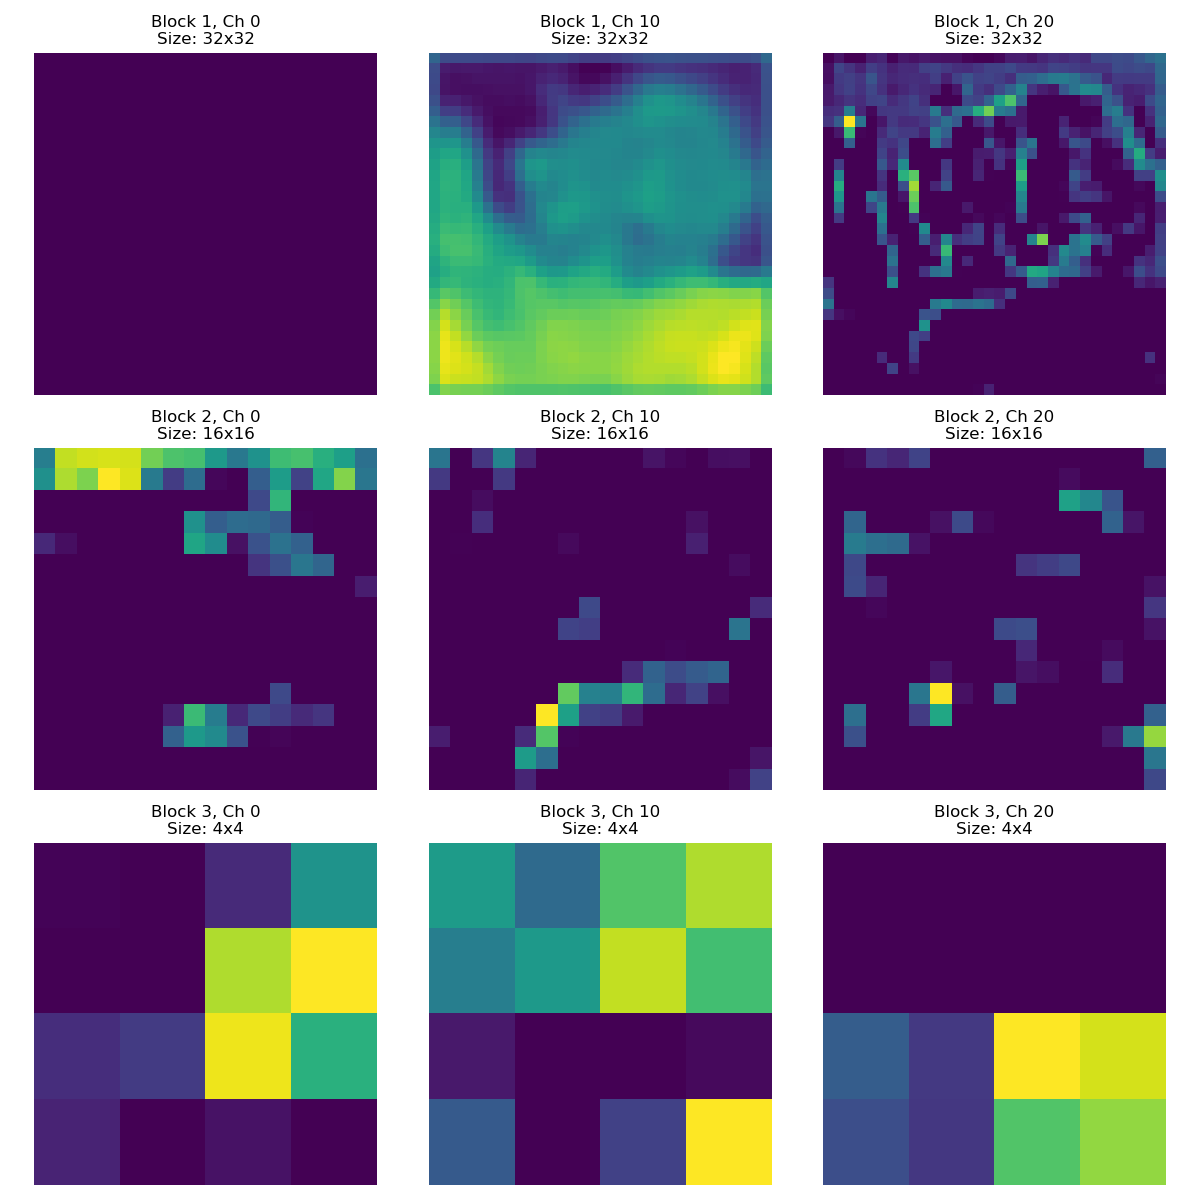
\includegraphics[width=0.8\textwidth]{assignment_1/report/images/feature_maps_visualization.png} 
    \caption{Visualization of  feature maps across 3 convolutional blocks}
    \label{figure_1}
\end{figure}